\chapter{От симулятора к дрону}\label{ch:k-dronu}

Этот урок короткий и осторожный. Настоящий дрон весит, крутит винты и может ударить. Всё, что ниже, делайте только вместе с учителем или взрослым и только после того, как шоу прошло проверку на экране.

\begin{opasno}[Правила первого полёта]
\begin{itemize}
  \item Первый полёт делайте \textbf{одним дроном}, а не всем строем.
  \item Рядом с ковриком не должно быть людей. Те, кто наблюдает, стоят за границей зоны.
  \item Рука лежит на красной кнопке \knopka{Аварийная посадка} или на клавише \klavisha{Esc}.
  \item Шаги \kod{circle} и \kod{code_z} на живом дроне \textbf{ещё не летали}. Если они есть в шоу, будьте особенно осторожны.
\end{itemize}
\end{opasno}

\section{Цепочка перед полётом}

\begin{figure}[H]
  \centering
  % Цепочка перед полётом
\begin{tikzpicture}[font=\sffamily\small, node distance=6mm,
  stp/.style={draw=accent, thick, rounded corners=2pt, fill=accentsoft, minimum height=9mm, minimum width=29mm, inner sep=3pt, align=center}]
  \node[stp] (a) {1. Проверить};
  \node[stp, right=of a] (b) {2. Загрузить};
  \node[stp, right=of b] (c) {3. Взвести};
  \node[stp, right=of c] (d) {4. Старт};
  \draw[-{Stealth}, accent, thick] (a) -- (b);
  \draw[-{Stealth}, accent, thick] (b) -- (c);
  \draw[-{Stealth}, accent, thick] (c) -- (d);
  \node[below=2mm of a, font=\scriptsize, text=inkgray, align=center] {симуляция,\\нет ошибок};
  \node[below=2mm of b, font=\scriptsize, text=inkgray, align=center] {программа\\уходит в дрон};
  \node[below=2mm of c, font=\scriptsize, text=inkgray, align=center] {разрешает\\старт};
  \node[below=2mm of d, font=\scriptsize, text=inkgray, align=center] {после вашего\\подтверждения};
  \node[draw=stopedge, thick, rounded corners=2pt, fill=stopfill, minimum height=9mm, inner sep=5pt, below=17mm of $(b)!0.5!(c)$, text=stopedge, font=\sffamily\small\bfseries] (r) {Аварийная посадка \;\klavisha{Esc}};
  \node[font=\scriptsize, text=inkgray, right=3mm of r, align=left] {всегда на экране,\\работает в любой момент};
\end{tikzpicture}

  \caption{Четыре шага перед полётом и красная кнопка, которая работает всегда.}\label{fig:chain}
\end{figure}

\begin{enumerate}
  \item \textbf{Проверить.} Нет ошибок и нет неожиданных замечаний.
  \item \textbf{Загрузить.} Программа каждого дрона превращается в набор шагов и уходит в выбранные дроны. Приложение откажет, если высота выше лимита, ожидание дольше 60\,с, батарея ниже 7,0\,В или дрон стоит не на своём месте. Подсказка рядом с кнопкой объясняет причину.
  \item \textbf{Взвести.} Разрешает старт. Взвод можно снять ещё одним щелчком.
  \item \textbf{Старт.} Появляется вопрос с подтверждением. Только после него дроны полетят.
\end{enumerate}

Цепочка сама подсказывает следующую кнопку. Если дронов на связи нет, шоу можно писать, смотреть и проверять, но не лететь: кнопки загрузки и старта остаются серыми, и подсказка объясняет причину.

\section{Связь и дроны}

Дроны сами находят компьютер в сети. В верхней панели нажмите на значок связи, выберите сетевой адаптер, подключённый к Wi-Fi дронов (адрес вида 192.168.13.x), и нажмите \knopka{Слушать}. Связь работает только в приложении, а не в браузере.

\begin{figure}[H]
  \centering
  \fbox{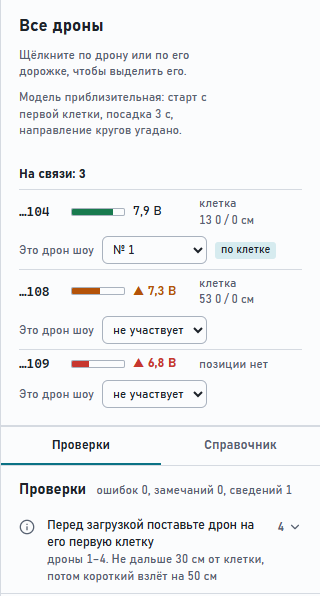
\includegraphics[width=0.42\textwidth]{figures/c_live.png}}
  \caption{Три придуманных дрона на связи. У каждого заряд батареи, клетка коврика и выбор «Это дрон шоу». Ниже список проверок.}\label{fig:live}
\end{figure}

\textbf{Роли.} Приложению нужно знать, какой живой дрон какому дрону шоу соответствует. Номер подставляется сам: если живой дрон стоит на первой клетке дрона N из шоу и больше никого на ней нет, приложение решает, что это дрон N (метка «по клетке»). Если два дрона стоят на одной клетке, номер остаётся пустым. Свой выбор главнее автоматического. Дрон, у которого выбрано «не участвует», в шоу не летит. Давно молчащие дроны уходят в архив списка.

\section{Батарея}

\begin{itemize}
  \item Ниже 7,4\,В карточка дрона становится янтарной: лучше заменить батарею.
  \item Ниже 7,0\,В взлёт запрещён: загрузка откажет, порог снизить нельзя.
\end{itemize}

\section{Позиция по коврику}

Дрон двигается по коврику \emph{абсолютно}: он летит к клетке, откуда бы ни стартовал. Поэтому ему нужна позиция, и стоять он должен рядом с первой клеткой своего движения.

\begin{enumerate}
  \item Поставьте дрон на коврик на первую клетку, в которую шоу его посылает (какая это клетка, пишет сведение в проверках). Лучше прямо на неё.
  \item Сделайте короткий взлёт на 50\cm, чтобы дрон получил позицию. Позиция остаётся после посадки.
  \item Убедитесь, что в списке дронов появилась клетка и она нужная.
  \item Не переносите дрон между загрузкой и стартом: позиция проверяется при старте ещё раз.
\end{enumerate}

Без позиции дрон прервёт миссию с движением по клеткам примерно через 3 секунды, не взлетев. Одна калибровка позицию не даёт.

\begin{vnimanie}[Две цифры про первую клетку]
Проверка допускает расстояние до первой клетки до 200\cm, а в подсказке приложение пишет «не дальше 30\,см». Берите строгое число: ставьте дрон точно на клетку.
\end{vnimanie}

\section{Что полетит не так, как на экране}

\begin{itemize}
  \item \textbf{Точность}: дрон ошибается на 10--15\cm, перелёт до 20\cm.
  \item \textbf{Посадка}: на экране 3 секунды, на дроне шаг посадки времени не добавляет.
  \item \textbf{Круги}: на дроне шаг \kod{circle} длится в \kod{count} раз дольше.
  \item \textbf{Старт}: симулятор считает, что дрон стоит под первой клеткой на земле. Живой дрон стоит там, где вы его поставили.
\end{itemize}

\section{Аварийная посадка}

Красная кнопка внизу справа и \klavisha{Esc} отправляют дронам команду посадки. Она работает, пока дрон взведён или летит. Если пропала связь или произошла ошибка, приложение само отправляет посадку и пишет в журнал, что случилось. Но не рассчитывайте на это: следите за полётом.
